\chapter{Tensor Structured Coupled Cluster}
\label{ch:tcc} 
The discussion presented in this section based on our published work, see 
Ref.~\cite{schutski2017tensor}, and also on new results intended for another 
publication.

\section{Motivation}
\label{sec:Introduction} 
Having seen that both strong and weak electronic correlation can be captured 
by methods based on the Projected Hartree-Fock, let us now turn to another 
powerful family of theories to solve many-body problems, namely, Coupled 
Cluster (CC). Since their introduction in the nuclear 
physics,\cite{coester1958bound, coester1960short} Coupled Cluster methods 
quickly became a "gold standard" of quantum chemistry due to their exceptional 
ability to capture weak electronic correlation, while having polynomial 
computational cost in basis size. Another attractive properties of most CC 
methods are size consistency and size extensivity.\cite{pople1978electron, 
bartlett1978many, crawford2000introduction, bartlett2007coupled} 

{\color{red} Insert 2 paragraphs here where accuracy of Coupled Cluster is 
discussed. Take it from Irek.}

Coupled Cluster methods parameterize the solution in terms of a reference 
wavefunction $| 0 \rangle$ and a set of excitation operators:
\begin{equation}
 | \phi \rangle  = \exp({}^1\hat{T} + {}^2\hat{T} + {}^3\hat{T} + \ldots) | 0 
\rangle
\end{equation}
where ${}^1\hat{T}, {}^2\hat{T}, \ldots$ are appropriate single, double, and 
higher order excitations from the reference state $| 0 \rangle$ (usually a HF 
solution). The method with n-body excitations is exact for n-electron systems. 
In practice, however, the excitation operator is truncated at doubles due to 
high computational cost, leading to Coupled Cluster with Singles and Doubles 
methods (CCSD).\cite{purvis1982full} Higher order excitations can be included 
approximately with the help of perturbation theory, such as in the highly 
accurate and widely used Coupled Cluster with Singles, Doubles and 
perturbative Triples (CCSD(T)) approach.\cite{bartlett1990non}

CC methods are also distinguished by the form of excitation operators, 
leading to Restricted (RCCSD),\cite{scuseria_ccsd} Unrestricted (UCCSD) and 
General (GCCSD) Coupled Cluster, in the same way as Hartree-Fock methods can be 
classified. A further analogy to HF method is that the solution of conventional 
Restricted Coupled Cluster method has proper $S^{2}$ and $S^{z}$ symmetry, but a 
wrong energy in case of strong correlation.

\begin{figure}[!ht]
\centering
 \rule{0.8\textwidth}{2cm}
 \caption{Restricted Coupled Cluster with Singles and Doubles in different 
correlation regimes. System: $N_{2}$, cc-pVDZ basis set. Exact is FCI solution.}
\end{figure}

This failure of Restricted CCSD in strong correlation regime is one (and 
probably most serious) downside of traditional Coupled Cluster theory. Another 
drawback is a steep growth of computational cost,\cite{noga1987full, 
scuseria1989coupled} which scales as $O(N^6)$ for CCSD, $O(N^7)$ for CCSD(T), 
and $O(N^8)$ for CCSDT, where $N$ is a size of basis. In the following we set 
to tackle both of these problems of conventional Coupled Cluster theory with 
tensor decompositions.

\section{Restricted Coupled Cluster with Singles and Doubles}
Let us start by describing the traditional Restricted Coupled Cluster 
\emph{ansatz}.\cite{bartlett2007coupled} The wavefunction is 
parameterized by an excitation operator $T$ and a single reference 
determinant $| 0 \rangle$:

\begin{equation}
 | \phi \rangle  = \exp(\hat{T}) | 0 \rangle = \exp({}^1\hat{T} + {}^2\hat{T} + 
{}^3\hat{T} + \ldots) | 0 \rangle
\end{equation}

In restricted version of Coupled Cluster theory excitation operators are spin 
adapted combinations of creation and annihilation operators of the form:

\begin{equation}
\begin{split}
 E_{i}^{a} & = \frac{1}{2} \cdot (a_{a, \uparrow}^{\dagger} a_{i, \uparrow} + 
a_{a, \downarrow}^{\dagger} a_{i, \downarrow}) \\
 {}^{1}\hat{T} & = {}^{1}T_{i}^{a} E_{i}^{a} \\
 {}^{2}\hat{T} & = \frac{1}{2} ~~ {}^{2}T_{ij}^{ab} E_{i}^{a} E_{j}^{b} \\
 \ldots
\end{split}
\end{equation}

Here indices $i, j$ represent particles, $a, b$ represent holes and summation 
is implied over repeated indices. The quantities denoted by $T$ are 
excitation amplitude tensors, e. g. two, four or higher dimensional arrays of 
numbers.

The excitation operator is truncated to a specific level, the most widely used 
choice being doubles, e. g. ${}^{2}\hat{T}$, leading to RCCSD model. If singles 
are omitted as well, we end up with RCCD method. With a wavefunction in the 
chosen form the Schr{\"o}edinger equation is

\begin{equation}
 H \exp(\hat{T}) |0 \rangle = E \exp(\hat{T}) |0 \rangle
\end{equation}

This equation is usually solved projectively by multiplying both sides of the 
expression by $\exp(-\hat{T})$. 
\begin{equation}
 \exp(-\hat{T}) H \exp(\hat{T)} | 0 \rangle = \bar{H} | 0 \rangle = E | 0 
\rangle
\label{eq:cc_lhs}
\end{equation}

From equation \ref{eq:cc_lhs} the energy can be extracted as an expectation 
value of the transformed Hamiltonian $\bar{H}$:

\begin{equation}
 E = \langle 0 | \bar{H} | 0 \rangle
\end{equation}

To obtain excitation amplitudes, the similarity transformed Hamiltonian 
is projected onto the set of excited determinants on the left.
Denoting these determinants as $\langle {}^{1}Z |$, $\langle {}^{2}Z|$
for single, double etc. excitations, one comes to a set of equations

\begin{equation}
\begin{cases}
 \langle {}^{1} Z_{i}^{a} | \bar{H} | 0 \rangle = {}^{1}R_{i}^{a} = 0 \\
 \langle {}^{2} Z_{ij}^{ab} | \bar{H} | 0 \rangle = {}^{2}R_{ij}^{ab} = 0 \\
 \ldots
\end{cases}
\label{eq:cc_residuals}
\end{equation}

where for every excited determinant the corresponding value of the residuals 
$R$ is zero. Residual equations are polynomial in the excitation amplitude 
tensors ${}^{1}T_{i}^{a}$, ${}^{2}T_{ij}^{ab}$ etc.

A common way of solving Eqn. \ref{eq:cc_residuals} is to split residual 
expressions into left and right hand sides to extract amplitudes. One such 
splitting is
\begin{subequations}
\begin{align}
 {}^{1}T_{i}^{a} &= {}^{1}D_{i}^{a} ~ {}^{1}G_{i}^{a}({}^{1}T, {}^{2}T), \\
{}^{2}T_{ij}^{ab} &= {}^{2}D_{ij}^{ab} ~ {}^{2}G_{ij}^{ab}({}^{1}T, {}^{2}T), 
\label{eq:cc_amplitude_equations_b}
\end{align}
\label{eq:cc_amplitude_equations}
\end{subequations}
Here, ${}^1D$ and ${}^2D$ are orbital energy
denominator tensors constructed from diagonal elements of the Fock matrix
$F$:

\begin{subequations}
\begin{align} {}^1D_i^a &= \frac{1}{F_a^a - F_i^a}, \\
{}^{2}D_{ij}^{ab} &= \frac{1}{F_{a}^{a} + F_{b}^{b} - F_{i}^{i} -
F_{j}^{j}}.
\end{align}
\label{eq:cc_denom_definition}
\end{subequations} 

Amplitude equations \ref{eq:cc_amplitude_equations} are solved by iterations 
until a fixed point is found.

Solving amplitude equations is computationally demanding, and determines a 
very steep cost of CC approach. For example, the evaluation of 
the right hand side of Eq. \ref{eq:cc_amplitude_equations_b} requires 
$O(N^6)$ summations and multiplications per iteration, hence RCCSD method has 
$O(N^6)$ cost. The root of this problem is the need to manipulate high order 
tensors representing the Hamiltonian and excitation amplitudes. This problem, 
however, can be circumvented by using novel techniques of tensor 
decompositions coming from multilinear algebra,\cite{kolda2009tensor} as we 
will show. 

\section{Tensor Contractions and the Cost of Coupled Cluster}
Let us discuss the cost of Coupled Cluster methods. The amplitude update 
equation in RCCD, the simplest representative of CC family, is:

\begin{equation}
\begin{split}
T^{ab}_{ij} & = D^{ab}_{ij} \cdot (- V^{ab}_{ij} \\
& + \sum_{k \neq i} F^{k}_{i} T^{ab}_{kj}
+  \sum_{k \neq j} F^{k}_{j}  T^{ab}_{ik}
- \sum_{c \neq a} F^{a}_{c}  T^{bc}_{ji}
- \sum_{c \neq b} F^{b}_{c}  T^{ac}_{ij} \\
& - T^{cd}_{ij}  V^{ab}_{cd}
+ T^{ac}_{ik}  V^{bk}_{cj} 
+ T^{ac}_{ki}  V^{bk}_{jc} 
+ T^{ac}_{kj}  V^{bk}_{ci} 
+ T^{bc}_{jk}  V^{ak}_{ci}\\
&+ T^{bc}_{ki}  V^{ak}_{cj} 
+ T^{bc}_{kj}  V^{ak}_{ic}
- 2 T^{ac}_{ik}  V^{bk}_{jc}
- 2 T^{bc}_{jk}  V^{ak}_{ic}
- T^{ab}_{kl}  V^{kl}_{ij} \\
&- T^{ab}_{ik}  T^{cd}_{lj}  V^{kl}_{cd} 
- T^{ab}_{kj}  T^{cd}_{il} V^{kl}_{dc}
- T^{ab}_{kl}  T^{cd}_{ij} V^{kl}_{cd}
- T^{ac}_{ij}  T^{bd}_{kl}  V^{kl}_{dc}
-  T^{ac}_{ik}  T^{bd}_{lj} V^{kl}_{dc} \\
&- T^{ac}_{ki}  T^{bd}_{jl} V^{kl}_{dc}
- T^{ac}_{ki}  T^{bd}_{lj} V^{kl}_{cd}
- T^{ac}_{kj}  T^{bd}_{li} V^{kl}_{dc}
-  T^{ac}_{kl}  T^{bd}_{ji} V^{kl}_{cd}
+ 2    T^{ab}_{ik} T^{cd}_{lj}  V^{kl}_{dc}\\
&+ 2    T^{ab}_{kj} T^{cd}_{il}  V^{kl}_{cd}
+ 2    T^{ac}_{ij} T^{bd}_{kl}  V^{kl}_{cd}
+ 2    T^{ac}_{ik}  T^{bd}_{jl}  V^{kl}_{dc}
+ 2    T^{ac}_{ik}  T^{bd}_{lj}  V^{kl}_{cd}  
+ 2    T^{ac}_{ki} T^{bd}_{jl}  V^{kl}_{cd}\\
&+ 2    T^{ac}_{kl} T^{bd}_{ji}  V^{kl}_{dc}
- 4    T^{ac}_{ik} T^{bd}_{jl}  V^{kl}_{cd})
\end{split}
\label{eq:ccd_amplitude_equation}
\end{equation}

Here $V$ is electron interaction tensor in the molecular orbital basis (Dirac 
ordered), $F$ is a Fock matrix, and $D$ is an orbital energy denominator. Most 
of the terms on the right hand side of Eqn.~\ref{eq:ccd_amplitude_equation} are 
numerically expensive to evaluate. For example, the sixth 
contraction in Eqn.~\ref{eq:ccd_amplitude_equation} is
\begin{equation}
 \tau^{ab}_{ij} = T^{ac}_{ik}  V^{bk}_{cj}
 \label{eq:ccd_intermediate_example}
\end{equation}
This expression requires $O(N^6)$ multiplications and additions, as for every 
of $N^4$ elements in the intermediate $\tau$ one has to calculate $N^2$ products
and sums. To facilitate the discussion and the estimates of cost let us 
introduce a graphical notation for tensors:

\begin{equation}
\vcenter{\hbox{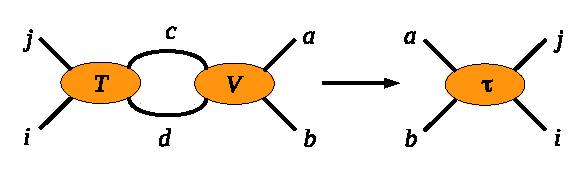
\includegraphics[width=0.6\textwidth]{figures/cc_contraction_1}}}
.
\label{fig:cc_contraction_1}
\end{equation}

In the graphical notation we represent tensors by shapes, and their indices by 
lines. Open lines mean free indices, and connected lines denote contraction 
over respective indices. One can then estimate the cost of the contraction as 
$N$ to the power of the number of connected lines plus the number of 
open lines if each index had a size proportional to $N$. The cost scales 
as $N^6$ in this example. For more examples of this notation please see the 
Appendix~\ref{sec:Appendix}. We will omit index letters on further diagrams.

The very same contraction can be done with lesser effort if electron 
interaction tensor is approximated by a well known\cite{beebe1977, 
vahtras1993integral, boman2008method, sierka2003fast} Resolution of Identity 
(RI) decomposition, also known as Density Fitting (DF):
%
\begin{equation} V^{pq}_{rs} \approx \sum_{\alpha \alpha^{\prime}} 
U_{pr}^{\alpha}
D_{\alpha,\alpha^{\prime}} \tilde{U}_{qs}^{\alpha^{\prime}},
\label{eq:ri_decomposition}
\end{equation}
Here $U$ and $\tilde{U}$ are three index integrals and $D$ is a generalized 
overlap.\cite{ahmadi1995coulomb}. It is well known that the 
error of this approximation decreases exponentially with the 
size of auxiliary basis $\{ \alpha \}$, called the rank of RI, and that 
negligible errors are attained 
with $dim(\{ \alpha \}) = r_{RI} = O(N)$.\cite{beebe1977, sierka2003fast} 
Diagrammatically, Eqn.~\ref{eq:ri_decomposition} is

\begin{equation}
\vcenter{\hbox{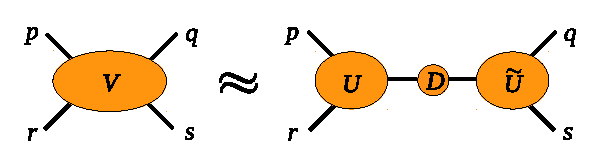
\includegraphics[width=0.6\textwidth]{figures/ri_decomposition}}}
.
\label{fig:ri_decomposition}
\end{equation}

By using the RI approximation to the electron interaction tensor the 
intermediate in Eqn.~\ref{fig:cc_contraction_1} can be formed at $O(N^5)$ cost, 
as shown on the diagram below:

\begin{equation}
\vcenter{\hbox{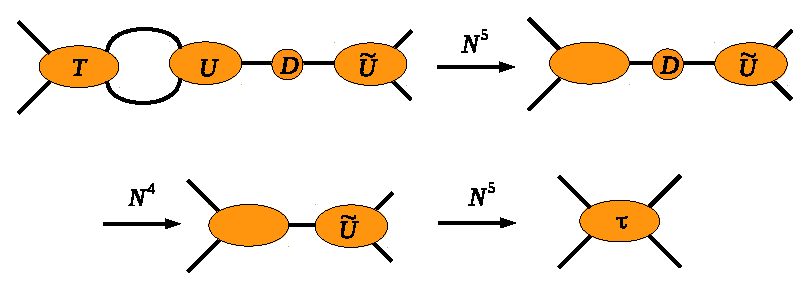
\includegraphics[width=0.6\textwidth]{figures/cc_contraction_2}}}
.
\label{fig:cc_contraction_2}
\end{equation}

The RI decomposition has been used for a long time to reduce the
scaling of quantum chemistry algorithms, for example, in the RI-MP2
method.\cite{ayala1999linear, werner2003fast, izmaylov2008resolution} An 
important caveat is that, however, keeping the dimension of the auxiliary 
basis low, in this approximation one can only 
separate a pair of indices $p, r$ 
from another pair $q, s$ with negligible error, but not $p, q$ from $r, s$. 
In the latter case the rank of RI has to be $r_{RI} = O(N^2)$ instead of 
$r_{RI} = O(N)$ in the former case to provide equivalent error, and thus such 
approximation would be not useful. Those properties of RI are 
apparent from the form of the electron interaction operator:

\begin{equation}
%\begin{split}
 V^{pq}_{rs} = \int \frac{\phi^{\ast}_{p}(r_{1}) 
\phi^{\ast}_{q}(r_{2}) \phi_{r}(r_{1}) \phi_{s}(r_{2})}{| r_{1} - r_{2} |} 
dr_{1} dr_{2} \\ 
%& \approx \int \phi^{\ast}_{p}(r_{1}) \phi_{r}(r_{1}) \chi_{\alpha}(r_{1}) 
%dr_{1} 
%\int \phi^{\ast}_{q}(r_{2}) \chi_{s}(r_{2}) \psi_{\alpha^{\prime}}(r_{2}) 
%dr_{2} \\ & \cdot \int \frac{\chi_{\alpha}(r_{1}) 
%\chi_{\alpha^{\prime}}(r_{2})}{| r_{1} - 
%r_{2} |} dr_{1} dr_{2}
%\end{split}
\label{eq:ri_decomposition_integral}
\end{equation}
As Eqn.~\ref{eq:ri_decomposition_integral} shows a separation of variables 
between a pair of basis functions $p, r$ and $q, s$ is possible when the 
distance $|r_{1} - r_{2}|$ is large. In contrast, this is not true for pairs 
$p, q$ and $r, s$.

This limitation of RI decomposition does not allow cost reduction during the 
calculation of several terms in the ${}^{2}T$ equation of RCCD. For example, 
the evaluation of the intermediate of the form:
\begin{equation}
 \tau^{ab}_{ij} = - T^{cd}_{ij}  V^{ab}_{cd}
\end{equation}
does not benefit from RI decomposition of $V$.
\begin{equation}
\vcenter{\hbox{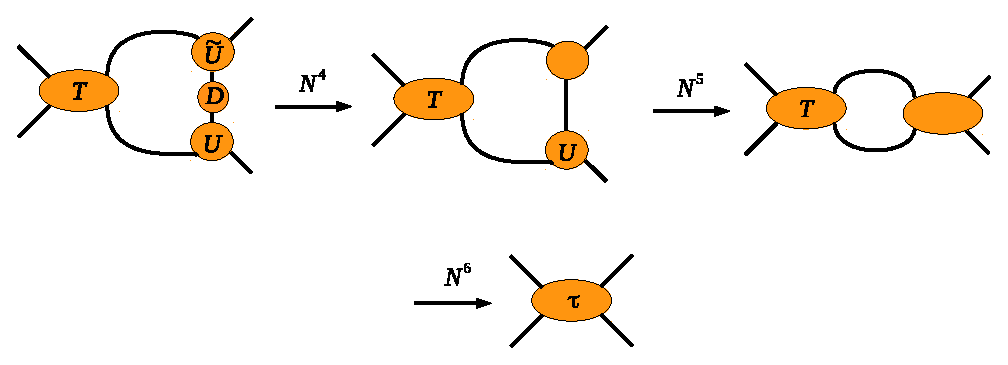
\includegraphics[width=0.8\textwidth]{figures/cc_contraction_3}}}
.
\end{equation}
Further approximations, however, can lead to reduced scaling, as we will show 
later.

\section{Tensor decompositions}
As was noted before, simple RI approximation may not always be flexible enough 
to reduce the computational cost of tensor contractions. To build a more 
applicable approximation of the interaction tensor we need to consider 
additional tensor decompositions. In this section we would only briefly list 
the decompositions we used, and refer the reader to original publications for 
technical details. The important information here is the structure of the 
described factorizations, which we demonstrate using tensor diagrams. Another 
important aspect is the alternating least squares method (ALS), as it can be 
used to calculate \emph{any} of the described decompositions and is a 
cornerstone of our factorized CC approaches.


\subsection{Canonical Polyadic Decomposition}
The canonical polyadic decomposition of a tensor is a decomposition of the 
form:\cite{de2006link}
%
\begin{equation}
T_{pqr\ldots} = \sum_\alpha a_p^\alpha \, b_q^\alpha \,
c_r^\alpha \ldots
\label{eq:cpd_definition}
\end{equation}

The CPD of a three index tensor is shown below diagrammatically.
\begin{equation}
\vcenter{\hbox{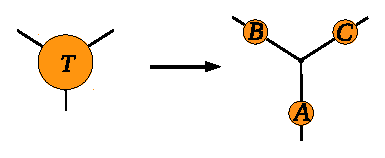
\includegraphics[width=0.4\textwidth]{figures/cp_decomposition}}}
.
\label{fig:cp_decomposition}
\end{equation}
%
This factorization can be seen as one of the generalizations of classic 
decompositions of matrices, such as QR, LU or Singular Value Decomposition, to 
higher order tensors.\cite{kolda2009tensor} The important difference, is, 
however, that no closed form algorithm to extract the CPD is known, and one has 
to rely on iterative optimization techniques to calculate the 
CP decomposition.\cite{sorber2013optimization} Substantial effort has been made 
by the mathematical community to develop approaches for doing so. We refer the 
reader to the corresponding reviews\cite{kolda2009tensor, 
sidiropoulos2016tensor} for further details. Typical algorithms are the 
alternating least squares (ALS),\cite{comon2009tensor} gradient descent by 
means of the method of Broyden, Fletcher, Goldfarb, and Shanno 
(BFGS), and nonlinear least squares (NLS) methods.\cite{sorber2013optimization}

\subsection{Tensor Hypercontraction}
The resolution of identity, which we considered before, can be combined with 
the canonical decomposition. Indeed, if three-index tensors in RI are further 
approximated by CPD one comes to a Tensor Hypercontraction introduced by 
Martinez \emph{et al.}\cite{hohenstein_thc1, hohenstein_thc2, hohenstein_thc3}
The THC is a decomposition of fourth order tensors of the form:
\begin{equation}
\begin{split} V_{pqrs} & = \sum_{\alpha \beta} W^{1}_{p,\alpha} W^{2}_{q, 
\alpha}
X_{\alpha, \beta} W^{3}_{r, \beta} W^{4}_{s, \beta} 
\end{split}
\label{eq:thc_definition}
\end{equation}
Diagrammatically, THC is
\begin{equation}
\vcenter{\hbox{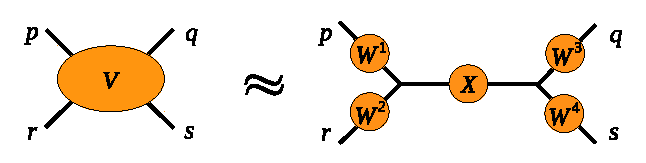
\includegraphics[width=0.5\textwidth]{figures/thc_decomposition}}
}
.\label{fig:thc_decomposition}
\end{equation}
THC can be seen as a further approximation to RI, which is apparent from the 
following sequence of diagrams:
\begin{equation}
\vcenter{\hbox{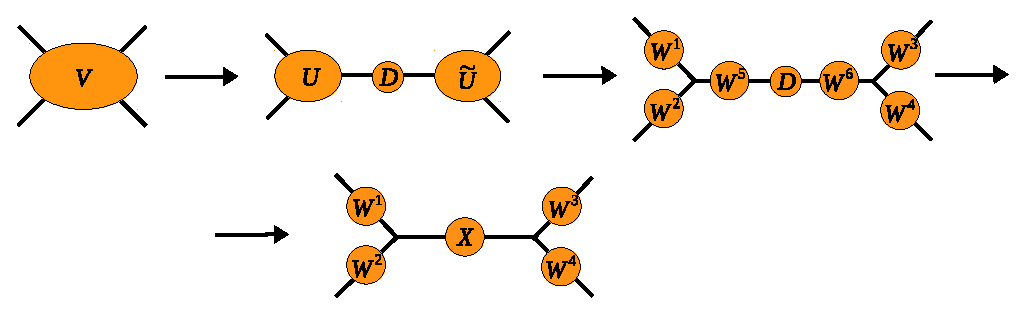
\includegraphics[width=0.8\textwidth]{figures/thc_cpd}}
}
.\label{fig:thc_cpd}
\end{equation}
 As those diagrams suggest, THC can be calculated in two steps: first, RI of 
the original tensor is calculated, and then CP decomposition of the three index 
tensors is obtained by means of an optimization 
algorithms.\cite{hohenstein_thc1} For the specific case of two 
electron integrals Martinez \emph{et al.} developed faster non-iterative 
methods where fixed real-space quadratures were used in place of factors $W^{1}, 
W^{2}, W^{3}, W^{4}$.\cite{hohenstein_thc3, hohenstein_cc2, parrish2013discrete} 
We also implemented direct optimization methods for calculating THC using 
alternating least squares and gradient descent in our 
work,\cite{schutski2017tensor} but found them inferior to the two step approach 
originally described by Martinez \emph{et al.}.\cite{hohenstein_thc1}

\subsection{Alternating Least Squares}
Let us now describe a general optimization method, which can be applied to 
calculate several tensor decompositions. We will show its derivation for the 
optimization of THC as was done in our original work,\cite{schutski2017tensor} 
but it can be equally used to compute CPD and, possibly, other decompositions.

We define an approximation to a four index tensor $V$ by its THC 
decomposition $\tilde{V}$
%
\begin{subequations}
\begin{align} \tilde{V}_{ijkl} &= \sum_{\alpha \beta} W^{1}_{p,\alpha} W^{2}_{q, 
\alpha} X_{\alpha, \beta} W^{3}_{r, \beta} W^{4}_{s, \beta} \\
\end{align}
\end{subequations}
%
The element-wise error can be written as
%
\begin{equation}
\Delta_{V} = V - \tilde{V},
\end{equation}
%
the square of the Frobenius norm of this tensor is a sum of its entries squared:
%
\begin{equation} f = \|\Delta_V\|^2 = \sum_{pqrs} \left(V^\ast_{pqrs} -
\tilde{V}^\ast_{pqrs}\right) \, \left(V_{pqrs} -
\tilde{V}_{pqrs}\right).
\label{eq:cost_function}
\end{equation}
%
Diagrammatically, this is
%
\begin{equation}
\vcenter{\hbox{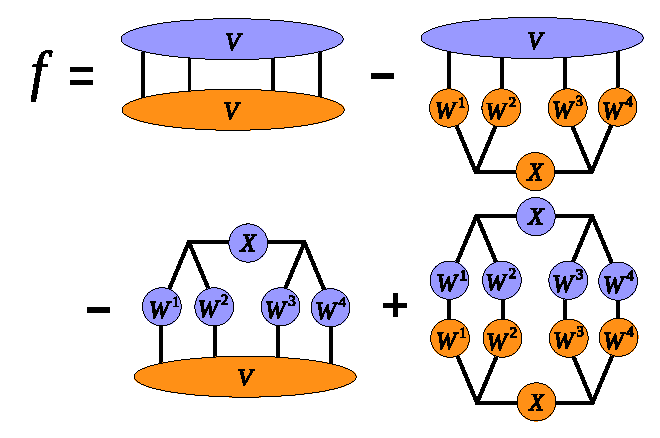
\includegraphics[height=38mm]{figures/cost_function}}}.
\label{fig:cost_function}
\end{equation}
%
where we denoted conjugated tensors by darker color. Clearly, the best possible 
THC approximation to $V$ will correspond to a minimum of the cost function $f$. 
Since $f$ is a real-valued analytic function, its derivatives with respect to 
possibly complex factors $W \in \{W^1, W^2, W^3, W^4, X\}$ are related by
$\frac{\partial f}{\partial W} = (\frac{\partial f}{\partial W^{\ast}})^{\ast}$.

In order to minimize the cost function, we proceed with the
calculation of its gradient, which can be easily done using
diagram~\ref{fig:cost_function}.  The partial derivative of $f$ with
respect to $W^1$ is
%
\begin{equation}
\vcenter{
\hbox{
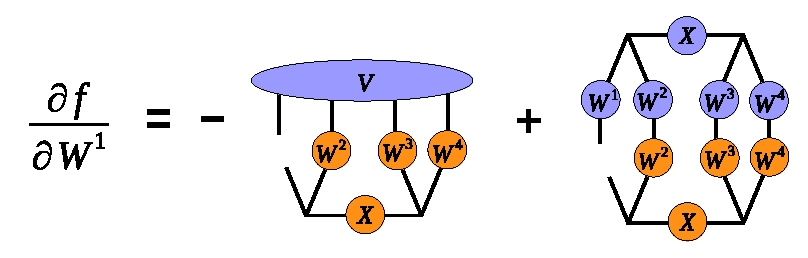
\includegraphics[width=0.8\textwidth]{figures/cost_function_dfdw1}}}
\label{fig:cost_function_partial}
\end{equation}
%
Likewise, partial derivatives of $f$ with respect to other factors are 
expressed by similar diagrams with those factors removed. Using the fact that 
$\frac{\partial f}{\partial W}$ is linear in $W^\ast$, we can contract all 
factors around $W^\ast$ into an environment matrix $A$, as shown in 
diagram~\ref{fig:least_squares_w1}, and set this derivative to zero:
%
\begin{equation}
\vcenter{\hbox{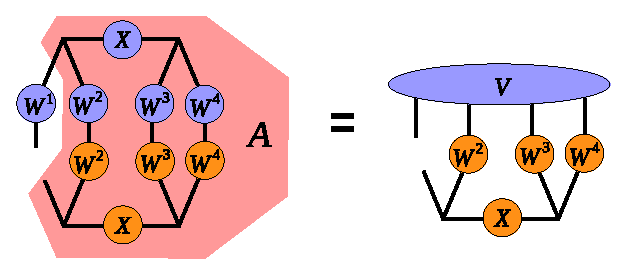
\includegraphics[width=0.6\textwidth]{figures/least_squares_w1}}}
\label{fig:least_squares_w1}
\end{equation}
%
We end up with a problem
%
\begin{equation}
A \cdot W^\ast = B.
\label{eq:least_squares_w1}
\end{equation}
%
The solution to Eq.~\ref{eq:least_squares_w1} can be
obtained by multiplying from the left by the inverse of $A$ (or a 
pseudoinverse, if $A$ is a rank-deficient matrix).  Finally, we arrive to an 
expression for ${W^{1}}^{\ast}$, which diagrammatrically is
%
\begin{equation}
\vcenter{
\hbox{
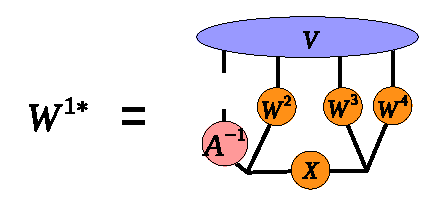
\includegraphics[width=0.4\textwidth]{figures/least_squares_w1_sol}}} .
\label{fig:least_squares_w1_sol}
\end{equation}
%
Let us estimate the cost of this procedure. We call the size of the 
auxiliary indices $\alpha, \alpha^{\prime}$ the rank of the THC 
decomposition ($r_\mathrm{THC}$). The construction of the environment 
matrix $A$ scales as $O(r_\mathrm{THC}^3)$, as does computing its generalized 
inverse. If each of the dimensions of $V$ equals $N$, then the cost of 
calculating ${W^1}^{\ast}$ scales as $O(N^4 \, r_\mathrm{THC})$. Updates for the
rest of the terms in the THC decomposition can be calculated similarly.

A simple iterative optimization algorithm can be built as follows.
First, the THC factors $W$ are initialized randomly.  For each factor,
an update is calculated as shown on diagram~\ref{fig:least_squares_w1_sol}, 
keeping the other factors fixed.  The process is iterated until convergence of 
the factors. We note that this procedure is, in fact, very similar to 
partial gradient descent and the Gauss-Siedel method.\cite{yoon1988lower} The 
resulting THC-ALS algorithm is listed below.

\begin{algorithm}[H]
  \caption{Alternating Least Squares}\label{code:thc_als}
  \begin{algorithmic}[1] 
  \Function{thc-als}{$V, r_\mathrm{THC}, \epsilon$}
  \State $I_{1},I_{2},I_{3},I_{4} \gets$ size($V$)
  \State $W^1, W^2, W^3, W^4, X \gets$ init\_random($I_{1}, I_{2}, I_{3}, 
I_{4}, r_\mathrm{THC}$) 
  \Repeat \ForAll {$W \in \{W^1, W^2, W^3, W^4,
X\}$}
  \State $A_{W} \gets $ get\_environment($W^1, W^2, W^3, W^4, X$)
  \LineComment{$O(r_\mathrm{THC}^3)$}
  \State $B_{W} \gets $ get\_rhs($V,
   W^1, W^2, W^3, W^4, X$) \LineComment{$O(N^4 \, r_\mathrm{THC})$ or
$O(N^2 \, r_\mathrm{RI} \, r_\mathrm{THC})$ with RI}
   \State $W_{new} \gets A^{-1} B$\Comment{$O(r_\mathrm{THC}^3)$}
   \EndFor
   \State $\Delta \gets \max_{W} \frac{\| W_{new} - W \|}{\|
W \|}$
   \State $W \gets W_{new}$ 
   \Until $\Delta > \epsilon$ 
   
   \Return $W^1, W^2, W^3, W^4, X$
    \EndFunction
  \end{algorithmic}
\end{algorithm}
%
The calculation of the right hand side of
Eq.~\ref{eq:least_squares_w1} dominates in the cost of THC-ALS,
scaling as $O(N^4 \, r_\mathrm{THC})$. A simple modification is
possible to reduce the cost of this step by one order of magnitude. If an
RI approximation to the original tensor $V$ is available from the beginning, as 
in the case of electron interaction, it can be used in place of $V$, leading to 
a faster algorithm. The diagram corresponding to 
Eq.~\ref{eq:least_squares_w1} then becomes
%
\begin{equation}
%\vcenter{\hbox{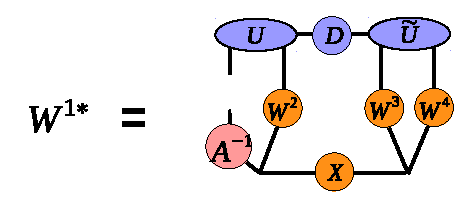
\includegraphics[height=20mm]{figures/least_squares_w1_sol_ri}}}
\label{fig:least_squares_w1_sol_ri}
\end{equation}
%
The cost of the expression above scales as $O(N^2 \,
r_\mathrm{RI} \, r_\mathrm{THC})$, because the contraction of a
fourth-index tensor $V$ with matrices $W$ is replaced by contractions
of two third-index tensors $U$ and $\tilde{U}$. We only need to
modify the function $get\_rhs()$ to build a lower scaling algorithm,
which we refer to as THC-ALS-RI.

Alternating least squares algorithms are simple and 
often robust,\cite{uschmajew2012local} but may take a large number of
iterations to converge.\cite{comon2009tensor} Particularly, we found that 
calculating THC decomposition with ALS directly is inferior than using a two 
step scheme mentioned earlier.\cite{schutski2017tensor} Nevertheless, ALS 
procedures can be derived for various decompositions, and are a cornerstone of 
our tensor structured Coupled Cluster.




\section{Appendix}
\label{sec:Appendix} 